% Source-derived chapter 14: Elimination of    \texorpdfstring{$\III^*$}{III*}-fibers
% Original source: no-enriques-surface-over-the-integers
\chapter{Elimination of    \texorpdfstring{$\III^*$}{III*}-fibers}
\label{no-enriques-surface-over-the-integers-chapter-14}
\source{no-enriques-surface-over-the-integers}

\begin{remark}[Source section]
\label{no-enriques-surface-over-the-integers-chapter-14-source}
\source{no-enriques-surface-over-the-integers}
\source{no-enriques-surface-over-the-integers}
This chapter reproduces the corresponding section of the retrieved
LaTeX source, including its definitions, statements, examples, and
proofs. It has not yet been translated into Lean.
\notready
\end{remark}

% The source section title was: Elimination of    \texorpdfstring{$\III^*$}{III*}-fibers
\mylabel{Elimination III*}

Let $Y$ is a non-exceptional Enriques surface over the ground field $k=\FF_2$, with constant Picard scheme.
We now exclude the $\III^*$-cases from the table in Proposition \ref{key reduction}.
We proceed in two steps, treating the case of multiple fibers first:

\begin{proposition}
\source{no-enriques-surface-over-the-integers}
\notready
\mylabel{no multiple III*}
There is no genus-one fibration  $\varphi:Y\ra\PP^1$ having a multiple  fiber with Kodaira symbol $\III^*$. 
\end{proposition}

\proof
Seeking a contradiction, we assume   that $\varphi^{-1}(\infty)$
is multiple with Kodaira symbol $\III^*$. The dual graph is:
\begin{equation}
\label{dual graph III*}
\source{no-enriques-surface-over-the-integers}
\begin{gathered}
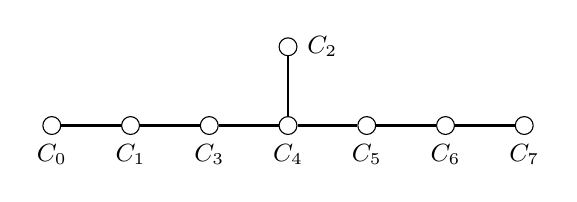
\begin{tikzpicture}
[node distance=1cm, font=\small]
\tikzstyle{vertex}=[circle, draw, fill=white, inner sep=0mm, minimum size=1.5ex]
\node[vertex]	(C0)  	at (1,0) [label=below:{$C_0$}] {};
\node[vertex]	(C1)	[right of=C0,  label=below:{$C_1$}]	{};
\node[vertex]	(C3)	[right of=C1,  label=below:{$C_3$}]	{};
\node[vertex]	(C4)	[right of=C3,  label=below:{$C_4$}]	{};
\node[vertex]	(C5)	[right of=C4,  label=below:{$C_5$}]	{};
\node[vertex]	(C6)	[right of=C5,  label=below:{$C_6$}]	{};
\node[vertex]	(C7)	[right of=C6,  label=below:{$C_7$}]	{};
\node[vertex]	(C2)	[above of=C4,  label=right:{$C_2$}]	{};
 
\draw[thick]    (C0)--(C1)--(C3)--(C4)-- (C5)--(C6)--(C7);
\draw[thick]    (C2)--(C4);
\end{tikzpicture}
\end{gathered}
\end{equation}
According to Proposition \ref{key reduction}, there is a genus-one fibration $\psi:Y\ra\PP^1$ having $\psi^{-1}(\infty)\cdot\varphi^{-1}(\infty)=4$.
We may assume that  $\psi^{-1}(\infty)$ has the largest number of irreducible components, among all fibers.
Choose a multiple fiber  $2F$  for $\psi$. After renumeration, we get $(F\cdot C_0)=1$.  
The connected curve $C_1+\ldots+C_7$ has dual graph $T_{2,3,4}$ and is thus contained in $\psi^{-1}(\infty)$. Its Kodaira
symbol must be $\III^*$, according to Proposition \ref{key reduction}. Let $C_0'\subset\psi^{-1}(\infty)$ be 
the additional component, which has $(C_0'\cdot C_1)=1$. From
$$
2\geq \varphi^{-1}_\ind(\infty)\cdot \psi_\ind(\infty) = (C_0+2C_1)\cdot C'_0 = (C_0\cdot C'_0) + 2
$$
we infer that $C_0$ and $C'_0$ are disjoint.
Thus  $C_0'+C_0+\ldots+ C_5$ supports a curve of canonical type $\I_2^*$.
Let $\tau:Y\ra\PP^1$ be the resulting genus-one fibration that has this curve as reduced fiber over $t=\infty$.
The fiber is multiple, because $\tau^{-1}_\ind(\infty)\cdot C_6=1$.
According to Proposition \ref{key reduction}, 
the fibers over $t=0,1$ have Kodaira symbol $\III$. Clearly, the curve $C_7$ belongs to one such fiber.
After applying an automorphism of $\PP^1$ we obtain
$$
\tau^{-1}_\ind(0)= C_7+C_7'\quadand \tau^{-1}_\ind(1) = R+R'.
$$
The dual graph for the configuration $C_0'+C_0+\ldots+C_7+C_7'+R+R'$ takes the following shape:
\begin{equation*}
\begin{gathered}
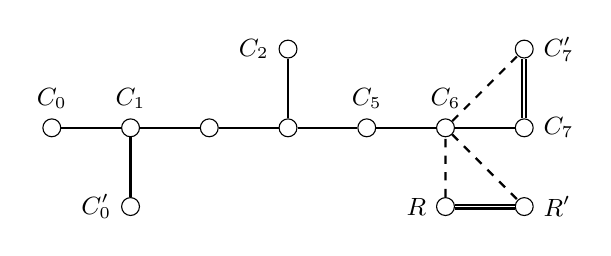
\begin{tikzpicture}
[node distance=1cm, font=\small]
\tikzstyle{vertex}=[circle, draw, fill=white, inner sep=0mm, minimum size=1.5ex]
\node[vertex]	(C0)  	at (1,0) 	[label=above:{$C_0$}] {};
\node[vertex]	(C1)			[right of=C0,  label=above:{$C_1$}]	{};
\node[vertex]	(C3)			[right of=C1,  label=above:{$$}]	{};
\node[vertex]	(C4)			[right of=C3,  label=above:{$$}]	{};
\node[vertex]	(C5)			[right of=C4,  label=above:{$C_5$}]	{};
\node[vertex]	(C6)			[right of=C5,  label=above:{$C_6$}]	{};
\node[vertex]	(C7)			[right of=C6,  label=right:{$C_7$}]	{};
\node[vertex]	(C2)			[above of=C4,  label=left:{$C_2$}]	{};
 
\node[vertex]	(C0')			[below of=C1,  label=left:{$C_0'$}]	{};
\node[vertex]	(C7')			[above of=C7,  label=right:{$C_7'$}]	{};
\node[vertex]	(R)			[below of=C6,  label=left:{$R$}]	{};
\node[vertex]	(R')			[below of=C7,  label=right:{$R'$}]	{};
 
\draw[thick]    (C0)--(C1)--(C3)--(C4)-- (C5)--(C6)--(C7);
\draw[thick]    (C2)--(C4);
\draw[thick]    (C1)--(C0');
\draw[thick,double]    (C7)--(C7');
\draw[thick,double]    (R)--(R');
\draw[thick,dashed]    (R)--(C6)--(R');
\draw[thick,dashed]     (C6)--(C7');
\end{tikzpicture}
\end{gathered}
\end{equation*}
The dashed edges indicate intersection numbers on which we can say the following:
First note that the intersection number $(R\cdot C_6)=1$   would lead to the configuration $C_0'+C_0+\ldots+C_7+R$, 
which contradicts   Proposition \ref{no I4*+R}.
For the same reason $(R'\cdot C_6)=1$  is impossible. 
On the other hand, we have 
$$
2= C_6\cdot\tau^{-1}(\infty) \geq C_6\cdot \tau^{-1}_\ind(1)=(C_6\cdot R)+(C_6\cdot R').
$$
After interchanging $R$ and $R'$ if necessary, we may assume that $(C_6\cdot R')=2$ and $(C_6\cdot R)=0$.
If follows that $R$ belongs to the fibers of  $\psi:Y\ra\PP^1$. 
According to Proposition \ref{possible configurations},   the    fiber $\psi^{-1}(\infty)$ 
with Kodaira symbol $\III^*$ must be multiple. 
Hence
$$
1=\varphi^{-1}_\ind(\infty)\cdot \psi^{-1}_\ind(\infty) = (2C_1\cdot C_0') =2,
$$
contradiction.
\qed

\begin{proposition}
\source{no-enriques-surface-over-the-integers}
\notready
\mylabel{no simple III*}
There is no genus-one fibration $\varphi:Y\ra\PP^1$ having a simple fiber with Kodaira symbol $\III^*$. 
\end{proposition}

\proof
Seeking a contradiction, we assume  that $\varphi^{-1}(\infty)$
is simple with Kodaira symbol $\III^*$, with dual graph as in \eqref{dual graph III*}.
According to Proposition \ref{key reduction}, 
there is another genus-one fibration $\psi:Y\ra\PP^1$ having $\psi^{-1}(\infty)\cdot\varphi^{-1}(\infty)=4$.
We may assume that  $\psi^{-1}(\infty)$ has the largest number of irreducible components, among all fibers.
Let $2F$ be one of the multiple fibers for $\psi$, such that $F\cdot \varphi^\inv(\infty)=2$.
After renumeration, we have  $(F\cdot C_2)=1$ or    $(F\cdot C_0)=(F\cdot C_7)=1$ or $(F\cdot C_1)=1$ or $(F\cdot C_0)=2$, with otherwise zero intersection numbers.
Our task is to rule out these four possibilities.

Suppose first that $(F\cdot C_2)=1$. Then $C_0+C_1+C_3+\ldots+C_7$ is a chain that is vertical with respect to $\psi$,
hence belongs to $\psi^{-1}(\infty)$. 
Its Kodaira symbol must be $\III^*$, by Propositions \ref{key reduction} and \ref{no I4*}.
We have $\psi^\inv_\red(\infty)= C_0+C_1+C_3+\ldots+C_7+R$,
with $(R\cdot C_4)=1$. This gives 
$$
4\geq \varphi^{-1}(\infty)\cdot \psi^\inv_\ind(\infty) = (4C_4+2C_2)\cdot 2R =8+ 4(C_2\cdot R)\geq 8,
$$
contradiction.

Next suppose that $(F\cdot C_0)=(F\cdot C_7)=1$. Then $C_1+\ldots+C_6$ has dual graph $T_{2,3,3}$ and is vertical with
respect to $\psi$, whence is contained in $\psi^\inv(\infty)$.
As above, the Kodaira symbol is $\III^*$, 
so $\psi^\inv_\red(\infty) = C_0'+C_1+\ldots+C_6+C_7'$, with $(C_0'\cdot C_1)=(C_7'\cdot C_6)=1$. Then
$$
4\geq \varphi^{-1}(\infty)\cdot \psi^\inv_\ind(\infty) = (C_0+2C_1+2C_6+C_7)\cdot(C_0'+C_7') \geq  4+  \sum (C_i\cdot C_j'),
$$
where the sum runs over $i,j\in \{0,7\}$. It follows that $C_0'\cup C_7'$ is disjoint from $C_0\cup C_7$.
Thus the curves $C_0'+C_0+\ldots C_7+C_7'$ forms a configuration as in Proposition \ref{no I4*+R}, contradiction.

We come to  the case $(F\cdot C_1)=1$, which is the most challenging.
The curve $C_2+\ldots+C_7$ has dual graph $T_{2,2,4}$ and is $\psi$-vertical, thus contained in $\psi^\inv(\infty)$.
Now the possible Kodaira symbols are  $\I_4^*$ or $\III^*$  or $\I_2^*$. 
The former was already discarded in  Proposition \ref{no I4*}. 
Suppose the symbol is $\III^*$.  It is simple by Proposition \ref{no multiple III*}, 
and with Proposition \ref{possible configurations} we infer that
also $C_0$ belongs to $\psi^\inv(\infty)$. Consequently  $\psi_\red^{-1}(\infty)=C_0+R+C_2+\ldots+C_7$ for some additional component $R$
with either $(R\cdot C_0)=(R\cdot C_3)=1$ or $(R\cdot C_0)=(R\cdot C_2)=1$.  In the former case
$$
4\geq \varphi^{-1}(\infty)\cdot \psi^\inv_\ind(\infty) = (C_0+2C_1+3C_3)\cdot 2R = 2 + 4(C_1\cdot R) + 6\geq 8,
$$
contradiction, and the latter case is treated analogously. So our fiber has Kodaira symbol $\I_2^*$,
and $\psi^\inv_\red(\infty)=C_2+\ldots+C_7+R$ for some additional component $R$ with $(R\cdot C_6)=1$. Now
$$
4\geq \varphi^{-1}(\infty)\cdot \psi^\inv_\ind(\infty) = (2C_1+ 2C_6)\cdot R = 2(C_1\cdot R) + 2.
$$
This gives $(C_1\cdot R)\leq 1$. But the case $(C_1\cdot R)=1$ yields a curve $R+C_1+C_3+\ldots+C_6$ of canonical type $\I_6$,
contradiction. Thus $C_1\cap R=\varnothing$.

According to Proposition \ref{key reduction}, $\psi$ has $\I_2^*+\III+\III$
as  configuration of fibers over rational points. The curve $C_0$ is $\psi$-vertical, and
we can assume $\psi^\inv_\ind(0)=C_0+C_0'$. Write $\psi^\inv_\ind(1)=D+D'$.
The dual graph for all our curves takes the following form:
\begin{equation*}
\begin{gathered}
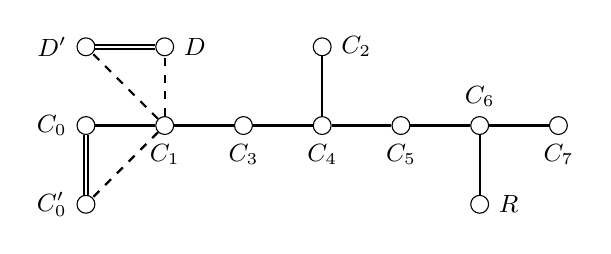
\begin{tikzpicture}
[node distance=1cm, font=\small]
\tikzstyle{vertex}=[circle, draw, fill=white, inner sep=0mm, minimum size=1.5ex]
\node[vertex]	(C0)  	at (1,0)  [		label=left:{$C_0$}] {};
\node[vertex]	(C1)	[right of=C0,	label=below:{$C_1$}] {};
\node[vertex]	(C3)	[right of=C1,	label=below:{$C_3$}] {};
\node[vertex]	(C4)	[right of=C3,	label=below:{$C_4$}] {};
\node[vertex]	(C5)	[right of=C4,	label=below:{$C_5$}] {};
\node[vertex]	(C6)	[right of=C5,	label=above:{$C_6$}] {};
\node[vertex]	(C7)	[right of=C6,	label=below:{$C_7$}] {};
\node[vertex]	(C2)	[above of=C4,	label=right:{$C_2$}] {};

\node[vertex]	(R)		[below of=C6, 	label=right:{$R$}] {};
\node[vertex]	(C0')	[below of=C0, 	label=left:{$C_0'$}] {};
\node[vertex]	(D)		[above of=C1, 	label=right:{$D$}] {};
\node[vertex]	(D')	[above of=C0, 	label=left:{$D'$}] {};

\draw[thick]    (C0)--(C1)--(C3)--(C4)-- (C5)--(C6)--(C7);
\draw[thick]    (C2)--(C4);
\draw[thick]    (R)--(C6);
\draw[thick,double]  (D)--(D');
\draw[thick,double]  (C0)--(C0');
\draw[thick,dashed]  (C1)--(C0');
\draw[thick,dashed]  (C1)--(D);
\draw[thick,dashed]  (C1)--(D');

\end{tikzpicture}
\end{gathered}
\end{equation*}
According to Proposition \ref{possible configurations}, the simple fiber $\varphi^\inv(\infty)$ with Kodaira symbol $\III^*$
must intersect each $(-2)$-curve on $Y$. It follows that  $C_1$ intersects $D$ and $D'$.
From
$4\geq \varphi^{-1}(\infty)\cdot \psi^\inv_\ind(1) = 2C_1\cdot (D+D')$
we infer $(C_1\cdot D)=(C_1\cdot D')=1$. Thus $D+C_0+\ldots+C_7+R$ forms a configuration as in Proposition \ref{no I4*+R}, 
again a contradiction.

It remains to deal with the case $(F\cdot C_0)=2$. Then $C_1+\ldots+C_7$ has dual graph $T_{2,3,4}$ and is vertical with respect to $\psi$,
whence contained in $\psi^\inv(\infty)$. Its Kodaira symbol must be $\III^*$, by Proposition \ref{key reduction}.
Write $\psi^\inv_\red(\infty)=C_0'+C_1+\ldots+C_7$ for some additional component $C_0'$ with $(C_0'\cdot C_1)=1$.
The fiber is simple, by Proposition \ref{no multiple III*}, so
$$
4=\varphi^\inv(\infty)\cdot \psi^\inv(\infty) = \varphi^\inv(\infty)\cdot C_0' = (C_0+ 2C_1)\cdot C_0' = (C_0\cdot C_0') +2.
$$
Whence $(C_0\cdot C_0')=2$, and $C_0+C_0'$ is a curve of canonical type, with Kodaira symbol $\I_2,\tI_2$ or $\III$. 
Let $\eta:Y\ra\PP^1$ be the
ensuing genus-one fibration. By Proposition \ref{key reduction}, we may assume that $\eta^{-1}(\infty)$ has 
symbol $\III^*$ or $\I_2^*$. In the former case Proposition \ref{no multiple III*} ensures that it is simple
so by  Proposition \ref{possible configurations} the configuration must be $\III^*+E_4+E_4$, contradiction.
In light of Proposition \ref{possible configurations}, the only remaining possible configuration is $\I_2^*+\III+\III$.
Without restriction $\eta_\ind^{-1}(0)=C_0+C_0'$ and $\eta_\ind^{-1}(1)=D+D'$. 
The curve  $C_2+\ldots+C_7$ has dual graph $T_{2,2,4}$ and thus belongs to $\eta^{-1}(\infty)$.
Let $R$ be the additional component.  The dual graph  of  our curves takes the following form:
\begin{equation*}
\begin{gathered}
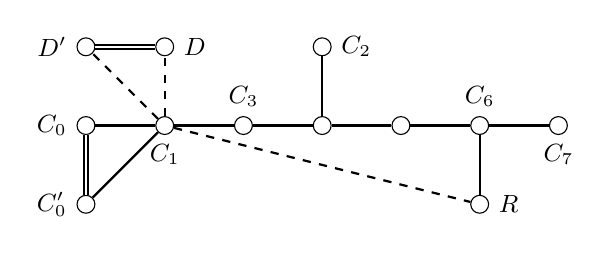
\begin{tikzpicture}
[node distance=1cm, font=\small]
\tikzstyle{vertex}=[circle, draw, fill=white, inner sep=0mm, minimum size=1.5ex]
\node[vertex]	(C0)  	at (1,0)  [		label=left:{$C_0$}] {};
\node[vertex]	(C1)	[right of=C0,	label=below:{$C_1$}] {};
\node[vertex]	(C3)	[right of=C1,	label=above:{$C_3$}] {};
\node[vertex]	(C4)	[right of=C3,	label=below:{}] {};
\node[vertex]	(C5)	[right of=C4,	label=below:{}] {};
\node[vertex]	(C6)	[right of=C5,	label=above:{$C_6$}] {};
\node[vertex]	(C7)	[right of=C6,	label=below:{$C_7$}] {};
\node[vertex]	(C2)	[above of=C4,	label=right:{$C_2$}] {};

\node[vertex]	(R)		[below of=C6, 	label=right:{$R$}] {};
\node[vertex]	(C0')	[below of=C0, 	label=left:{$C_0'$}] {};
\node[vertex]	(D)		[above of=C1, 	label=right:{$D$}] {};
\node[vertex]	(D')	[above of=C0, 	label=left:{$D'$}] {};

\draw[thick]    (C0)--(C1)--(C3)--(C4)-- (C5)--(C6)--(C7);
\draw[thick]    (C2)--(C4);
\draw[thick]    (R)--(C6);
\draw[thick,double]  (D)--(D');
\draw[thick,double]  (C0)--(C0');
\draw[thick]  (C1)--(C0');
\draw[thick,dashed]  (C1)--(D);
\draw[thick,dashed]  (C1)--(D');
\draw[thick,dashed]  (C1)--(R);
\end{tikzpicture}
\end{gathered}
\end{equation*}
We have 
$\eta^{-1}_\ind(0)\cdot \varphi^{-1}(\infty) = (C_0+C_0')\cdot 2C_1 =   2+2=4$.
If $\eta^{-1}(0)$ is simple, each multiple fiber $2F'$ for $\eta:Y\ra\PP^1$ has $(F'\cdot C_1) =1$, in contradiction to the previous 
paragraph. Thus $\eta^{-1}(0)$ is multiple, such that  $\eta^{-1}(\infty)\cdot\varphi^{-1}(\infty)= 8$.
If the fiber $\eta^{-1}(\infty)$ is multiple as well, we  get
$$
4=\eta_\ind^{-1}(\infty) \cdot \varphi^{-1}(\infty) = R\cdot (2C_1+2C_6) = 2(R\cdot C_1) + 2,
$$
hence $C_3+\ldots+C_6+R+C_1$ is a curve of canonical type $\I_6$, contradiction.
Thus $\eta^{-1}(\infty)$ is simple, whereas $\eta^{-1}(1)$ must be the second multiple fiber. The latter gives
$$
4=\eta^{-1}_\ind(1)\cdot\varphi^{-1}(\infty) = (D+D')\cdot 2C_1 = 2(D\cdot C_1)+2(D'\cdot C_1).
$$
According to Proposition \ref{possible configurations}, the fiber $\varphi^{-1}(\infty)$ intersects both $D$ and $D'$,
so we have  $(D\cdot C_1)=(D'\cdot C_1)=1$.  
Thus $D+C_1+\ldots+C_7$ gives a curve of canonical type $\III^*$. This gives a further fibration on $Y$, in which 
  the   fiber of type $\III^*$  must be simple, according to Proposition \ref{no multiple III*}. This gives
$$
4\leq (D+2C_1+\ldots+2C_6+C_7)\cdot\varphi^{-1}(\infty)=D\cdot 2C_1=2,
$$
contradiction.
\qed


%===========================================================
